\documentclass[12pt,a4paper,fleqn]{ctexart}

\usepackage{geometry}
\geometry{left=2.7cm,right=2.7cm,top=2.54cm,bottom=2.54cm}
\usepackage{setspace}
\setstretch{1.25}
\usepackage{graphicx}
\usepackage{booktabs}
\usepackage{longtable}
\usepackage{array}
\usepackage{chngcntr}
\usepackage{amsmath,amssymb}
\usepackage{caption}
\usepackage{subcaption}
\usepackage{float}
\usepackage{enumitem}
\usepackage[hidelinks]{hyperref}
\usepackage[backend=biber,style=gb7714-2015,sorting=none]{biblatex}

\addbibresource{refs/review.bib}
\setmainfont{Times New Roman}
\newfontfamily\TimesNewRoman{Times New Roman}
\newCJKfontfamily\HeiTiBold{SimHei}[AutoFakeBold=2.5]
\newCJKfontfamily\SongTiBold{SimSun}[AutoFakeBold=2.5]
\renewcommand{\contentsname}{目\hspace{2em}录}
\let\cite\supercite

\setlength{\mathindent}{2em}
\counterwithin{figure}{section}
\counterwithin{table}{section}
\numberwithin{equation}{section}
\renewcommand{\thefigure}{\arabic{section}-\arabic{figure}}
\renewcommand{\thetable}{\arabic{section}-\arabic{table}}
\renewcommand{\theequation}{\arabic{section}-\arabic{equation}}
\setlength{\heavyrulewidth}{1.5pt}
\setlength{\lightrulewidth}{0.5pt}
\setlength{\cmidrulewidth}{0.5pt}
\setlength{\bibhang}{2em}
\setlength{\bibitemsep}{0pt}
\DeclareCaptionLabelSeparator{twospace}{\hspace{2em}}
\DeclareCaptionFont{songtibold}{\SongTiBold\zihao{5}}
\captionsetup{
  justification=centering,
  singlelinecheck=false,
  labelsep=twospace,
  font={stretch=1.25},
  skip=6pt
}
\renewcommand*{\bibfont}{\songti\TimesNewRoman\zihao{5}\setstretch{1.25}}
\newcommand{\CaptionSource}[1]{%
  \if\relax\detokenize{#1}\relax
  \else
    \textsuperscript{\songti\zihao{6}[#1]}%
  \fi
}
\newcommand{\BiCaption}[3][]{%
  \caption{%
    {\SongTiBold\zihao{5}#2\CaptionSource{#1}}\\
    {\TimesNewRoman\bfseries\zihao{5}#3}%
  }%
}
\defbibheading{custombib}[\refname]{%
  \clearpage
  \addcontentsline{toc}{section}{#1}%
  \begin{center}
    {\heiti\zihao{3}#1}
  \end{center}
  \vspace{12pt}
}

\makeatletter
\renewcommand*\l@section{\@dottedtocline{1}{0em}{2.3em}}
\renewcommand*\l@subsection{\@dottedtocline{2}{1.5em}{3.2em}}
\renewcommand*\l@subsubsection{\@dottedtocline{3}{3.8em}{4.1em}}
\makeatother

\setcounter{tocdepth}{3}
\setcounter{secnumdepth}{3}

\AtBeginEnvironment{figure}{\captionsetup{position=bottom,labelfont=songtibold,textfont=songtibold}}
\AtBeginEnvironment{table}{\captionsetup{position=top,labelfont=songtibold,textfont=songtibold}}
\AtBeginEnvironment{tabular}{\songti\TimesNewRoman\zihao{5}\renewcommand{\arraystretch}{1.35}}
\AtBeginEnvironment{longtable}{\songti\TimesNewRoman\zihao{5}\renewcommand{\arraystretch}{1.35}}

\ctexset{
  section = {
    name = {第,章},
    number = \chinese{section},
    format = \centering\heiti\zihao{3},
    aftername = \hspace{1em},
    beforeskip = 24pt,
    afterskip = 12pt
  },
  subsection = {
    format = \heiti\zihao{4},
    aftername = \hspace{1em},
    beforeskip = 24pt,
    afterskip = 12pt
  },
  subsubsection = {
    format = \heiti\zihao{-4},
    aftername = \hspace{1em},
    beforeskip = 12pt,
    afterskip = 12pt
  }
}

\title{面向多视图几何重建的学习方法综述：以 VGG 团队为例}
\author{}
\date{}

\begin{document}

\begin{titlepage}
  \centering
  
\includegraphics[width=11.38cm]{figures/zjut.png}\par
  \vspace{0.6cm}
  {\centering\songti\zihao{1}《文献检索与论文写作》\par}
  \vspace{0.8cm}
  {\centering\songti\zihao{1}课程报告\par}
  \vspace{2.2cm}
  {\centering\heiti\zihao{3}题目：面向多视图几何重建的学习方法综述\par}
  \vspace{0.2cm}
  {\centering\heiti\zihao{3}——以 VGG 团队为例\par}
  \vspace{2.4cm}
  \begin{center}
    {\songti\zihao{-3}组\quad 长：\underline{\hspace{8.5cm}}\par}
    \vspace{0.6cm}
    {\songti\zihao{-3}组\quad 员：\underline{\hspace{8.5cm}}\par}
    \vspace{0.6cm}
    {\songti\zihao{-3}专\quad 业：\underline{\makebox[8.5cm][c]{计算机科学与技术}}\par}
    \vspace{0.6cm}
    {\songti\zihao{-3}班\quad 级：\underline{\makebox[8.5cm][c]{2023计算机科学与技术03}}\par}
    \vspace{0.6cm}
    {\songti\zihao{-3}提交日期：\underline{\makebox[7.8cm][c]{2026年5月}}\par}
  \end{center}
\vfill
\end{titlepage}

\clearpage
\addcontentsline{toc}{section}{摘要}
\begin{center}
  {\heiti\zihao{3}摘要}
\end{center}
\begingroup
\songti\zihao{-4}
\setstretch{1.25}
\parindent=2em
本文围绕多视图几何重建中的学习方法展开综述，聚焦 Oxford Visual Geometry Group（VGG）团队近五年的代表工作，分析该方向如何从传统结构恢复管线逐步演化到端到端学习、可微结构恢复以及统一前馈式几何预测框架。全文首先梳理传统 SfM/MVS 的任务定义与关键瓶颈，再从几何先验注入、对应关系学习、可微优化和统一几何表示四个层面总结 VGG 团队的研究主线，并结合 CoTracker、VGGSfM、VGGT 等代表性成果讨论学习方法对多视图几何重建范式的推动作用。最后，本文从鲁棒性、效率、统一性与可扩展性等角度，对该研究体系的特点、局限与未来趋势进行综合评述。

\par\noindent{\HeiTiBold\zihao{-4}关键词：}{\songti\zihao{-4}多视图几何重建，Structure-from-Motion，视觉几何，对应学习，VGG}
\endgroup

\clearpage
\addcontentsline{toc}{section}{ABSTRACT}
\begin{center}
  {\TimesNewRoman\zihao{3} LEARNING METHODS FOR MULTI-VIEW GEOMETRIC RECONSTRUCTION:}\\
  \vspace{0.2cm}
  {\TimesNewRoman\zihao{3} A REVIEW WITH THE VGG TEAM AS A CASE STUDY}
\end{center}

\begin{center}
  {\TimesNewRoman\zihao{3} ABSTRACT}
\end{center}
\begingroup
\TimesNewRoman\zihao{-4}
\setstretch{1.25}
\parindent=2em
This report reviews recent learning-based methods for multi-view geometric reconstruction, with a focus on the Oxford Visual Geometry Group (VGG) and its representative works over the last five years. We first revisit the classical SfM/MVS pipeline and its limitations in correspondence estimation, global consistency, and optimization efficiency. We then organize the VGG research line into four connected themes: geometric priors, correspondence learning, differentiable structure from motion, and feed-forward geometric prediction. Representative works such as CoTracker, VGGSfM, and VGGT are discussed to show how learning-based methods have progressively redefined the traditional multi-view geometry pipeline. Finally, we summarize the main characteristics, current limitations, and future opportunities of this research line.

\par\noindent{\TimesNewRoman\bfseries\zihao{-4}KEY WORDS: }{\TimesNewRoman\zihao{-4}multi-view geometry, structure from motion, visual geometry, correspondence learning, vgg}
\endgroup

\clearpage
\begingroup
\songti\TimesNewRoman\zihao{-4}
\setstretch{1.25}
\tableofcontents
\endgroup

\clearpage
\songti\zihao{-4}
\setstretch{1.25}
\setlength{\parindent}{2em}
\setlength{\parskip}{0pt}
\section{引言}

多视图几何重建旨在从无序或有序的多张图像中恢复场景的三维结构、相机内外参数以及与场景几何相关的中间表示，是从二维视觉观测走向三维世界理解的基础问题。对这一方向而言，核心任务并不只是“估计深度”或“回归位姿”，而是要在缺乏直接深度传感的前提下，利用跨视角投影关系，把分散的二维像素组织成一个几何上自洽、全局上一致、并可被下游任务复用的三维场景解释。传统方法通常遵循“特征提取与匹配、相机注册、三角化与光束法平差”的经典管线，其中 Bundle Adjustment 被视为保证全局一致性的关键环节\cite{triggs2000bundle,schoenberger2016colmap}。然而，这一管线高度依赖手工设计的特征与多阶段优化，面对弱纹理、遮挡、宽基线与大规模图像集合时，往往在鲁棒性、效率与泛化性上面临明显瓶颈\cite{wang2021deep2view,wang2024vggsfm}。

近五年，多视图几何重建逐步出现“学习化”趋势：研究者不再仅将深度网络作为传统流程的局部替代模块，而是尝试让网络直接参与几何对应、相机估计、全局优化乃至统一几何属性预测\cite{bhalgat2023lighttouch,karaev2024cotracker,wang2025vggt}。在这一演进过程中，学习方法的价值不只是“把某个模块做得更准”，而是重新回答三个相互关联的问题：如何获得更稳定的跨视角对应，如何让全局求解既保持几何约束又具备可学习性，以及如何把原本割裂的几何变量组织为可迁移的统一表示\cite{wang2024vggsfm,wang2025vggt}。也正因如此，多视图几何重建正在从传统的工程化流水线问题，逐渐转变为“几何结构如何被学习模型吸收和重组”的方法论问题。

在众多研究团队中，Oxford Visual Geometry Group（VGG）围绕这一主题形成了较为清晰且连续的研究主线。其工作并非对传统几何的简单替代，而是强调将多视图几何的结构性约束、对应关系与优化逻辑逐步转移到学习框架内部。从早期强调几何先验与任务设定的工作\cite{wu2020unsup3d,wang2021deep2view}，到关注点轨迹与跨视角关系建模的 CoTracker 系列\cite{karaev2024cotracker,karaev2025cotracker3}，再到将结构恢复系统整体可微化的 VGGSfM\cite{wang2024vggsfm}以及面向统一几何属性预测的 VGGT\cite{wang2025vggt}，VGG 团队的成果较完整地呈现了多视图几何重建“学习化”的方法演进。与只在单点任务上取得突破的工作相比，这条主线更适合被当作一个可分析的样本，因为它不仅包含代表性论文，更包含论文之间清晰的前后承接关系。

基于课程要求，本文选择“多视图几何重建中的学习方法”作为明确研究主题，以 VGG 团队为代表案例展开综述，而不是泛泛介绍整个团队的三维视觉工作。全文将重点回答以下问题：多视图几何重建这一方向为什么值得持续研究；它主要试图解决哪些核心问题；学习方法究竟改造了传统管线中的哪些关键环节；以及 VGG 团队的代表性成果如何形成一条层层递进的研究主线。通过这些问题，本文希望帮助读者同时理解“这个方向为什么重要”与“为什么 VGG 团队值得被单独综述”。

\subsection{研究背景与意义}

多视图几何重建广泛应用于自动驾驶、AR/VR、机器人导航、文化遗产数字化与三维内容生成等场景。相较依赖激光雷达或深度相机的主动感知方案，仅依赖普通 RGB 图像的方案具有设备廉价、部署灵活、成像分辨率高等优点，因此长期以来都是计算机视觉的重要研究方向\cite{schoenberger2016colmap,reizenstein2021co3d}。然而，图像到三维的恢复本质上是病态问题，必须借助跨视角几何约束、匹配一致性与全局优化，才能得到可信的相机与结构估计。

从应用层面看，多视图几何重建并不只是一个传统视觉任务，而是连接二维感知与三维世界理解的基础桥梁。在自动驾驶与机器人系统中，场景几何决定了障碍物定位、路径规划和交互安全；在 AR/VR 中，几何重建又直接关系到虚实对齐、遮挡关系与真实感渲染；在数字文化遗产保护与工业检测场景中，稳定而高精度的三维恢复则决定了后续建模、存档与测量分析的质量。因此，如何让仅依赖图像的三维重建方法变得更稳健、更高效、更易泛化，具有明确的工程价值与学术价值。

同时，该方向之所以长期具有研究吸引力，还在于它天然处于“物理规律”与“数据驱动学习”之间的交汇点。一方面，多视图几何由投影模型、相对运动和重投影误差等明确数学结构决定；另一方面，真实世界中的纹理缺失、反射、遮挡与动态变化，又使得纯解析方法难以覆盖全部复杂情形。也正是在这一张力下，学习方法才逐渐成为推动该方向继续发展的关键力量。

从当前技术发展背景看，这一方向之所以尤其值得在今天重新审视，还因为其正在与机器人感知、具身智能和三维内容生成等新需求发生更紧密的耦合。无论是需要实时空间理解的机器人系统，还是需要可编辑三维场景表示的生成式应用，都要求视觉系统不仅“看见”图像内容，更要获得可度量、可推理、可复用的场景几何结构。由此可见，多视图几何重建不只是一个传统问题的延续，而是在新的应用牵引下不断获得新意义的基础能力。

\subsection{核心关注点与研究难点}

该方向当前的核心难点主要包括：跨视角对应的不稳定性、增量式管线的误差累积、复杂场景下的泛化能力不足，以及大规模场景下优化成本过高等\cite{wang2021deep2view,karaev2024cotracker,wang2024vggsfm}。因此，如何在保持几何一致性的同时提高学习模型的表达能力与推理效率，构成了近年多视图几何重建研究的关键问题。

进一步细分，这些难点实际上对应多视图几何管线中的三个关键环节。第一是观测层，即如何从图像中获得高质量、可长期保持一致的对应关系；第二是求解层，即如何在相机恢复、三角化与全局优化阶段维持数值稳定与几何可解释性；第三是表示层，即如何让模型输出的几何结果既便于重建本身，也能够服务于深度估计、跟踪、视图合成和动态场景理解等下游任务。VGG 团队近五年的工作，恰恰可以被理解为分别围绕这三个环节逐步展开。

此外，近两年该方向又新增了一类重要问题，即统一性问题。过去多视图几何系统更倾向于“一个模块做一件事”，而当前越来越多方法开始尝试让同一模型同时处理相机参数、深度、点图和轨迹等多种属性\cite{wang2025vggt,wang2024dust3r,mast3r2024}。这意味着研究目标已经从“单模块精度提升”逐步转向“统一场景几何表示的构建”，这也是本文在综述中将 VGGSfM 和 VGGT 视为关键节点的重要原因。

若从更本质的层面概括，这一方向所面对的其实是三组长期存在的矛盾。其一是“局部观测有限”与“全局几何一致”之间的矛盾，即单个像素或局部匹配信息往往十分脆弱，但最终恢复出的相机和结构却必须满足全局自洽。其二是“显式优化可靠”与“计算代价高昂”之间的矛盾，即传统几何求解具有可解释性，却往往难以满足大规模和高效率需求。其三是“统一表示更具复用性”与“训练监督更复杂”之间的矛盾，即模型越希望一次性输出更多几何属性，就越需要更强的数据、监督和模型设计来维持一致性。当前多视图几何重建研究的核心关注点，正是在这三组矛盾之间寻找新的平衡。

\subsection{选择 VGG 团队作为综述对象的原因}

VGG 团队在该方向的工作具有三个适合作为综述案例的特征。第一，其研究主题高度集中，长期围绕几何先验、跨视角对应、SfM 系统学习化与统一几何表示展开。第二，其代表论文之间存在明显的递进关系，适合从“问题链条”而非“论文堆砌”角度组织综述。第三，其工作发表在 CVPR、ICCV、ECCV 等高水平会议，并普遍提供论文、项目页或代码，便于基于一级来源进行核实与写作\cite{bhalgat2023lighttouch,wang2024vggsfm,wang2025vggt}。

更重要的是，VGG 团队的方法路径具有较强的代表性和可分析性。与某些仅在单一任务或单一模型上取得突破的研究不同，VGG 团队的工作覆盖了数据、表征、几何求解与统一预测等多个层面，因而能够较完整地反映当前多视图几何重建学习化的总体趋势。与此同时，这条研究主线又保持了足够清晰的边界，使本文可以围绕“多视图几何重建中的学习方法”这一明确主题展开，而不会滑向泛泛的“某团队视觉研究综述”。

进一步说，选择 VGG 团队并不是因为它“覆盖面最广”，而是因为它恰好沿着本文最关心的研究链条持续推进。许多优秀团队也在多视图重建、NeRF、三维生成或视觉基础模型上取得了重要成果，但未必同时呈现出从几何先验、对应学习、系统求解到统一表示这一完整而连续的演进关系。相比之下，VGG 团队的价值在于：其代表性成果之间不仅共享主题，更共享一个可被清晰复原的问题推进逻辑，即前一阶段暴露出的瓶颈，往往直接构成后一阶段工作的出发点。

这使 VGG 团队特别适合作为课程综述对象。对于一篇强调“把研究内容讲清楚、把论文关系讲清楚、把发展逻辑讲清楚”的课程报告而言，最理想的样本不是论文数量最多的团队，而是能够帮助读者看见研究主线如何展开的团队。VGG 的研究路径恰好具备这种教学意义：它既足够前沿，能够反映近五年多视图几何重建的关键转向；又足够连贯，能够支撑从“为什么值得研究”一路分析到“未来可能如何发展”。

\begin{figure}[H]
  \centering
  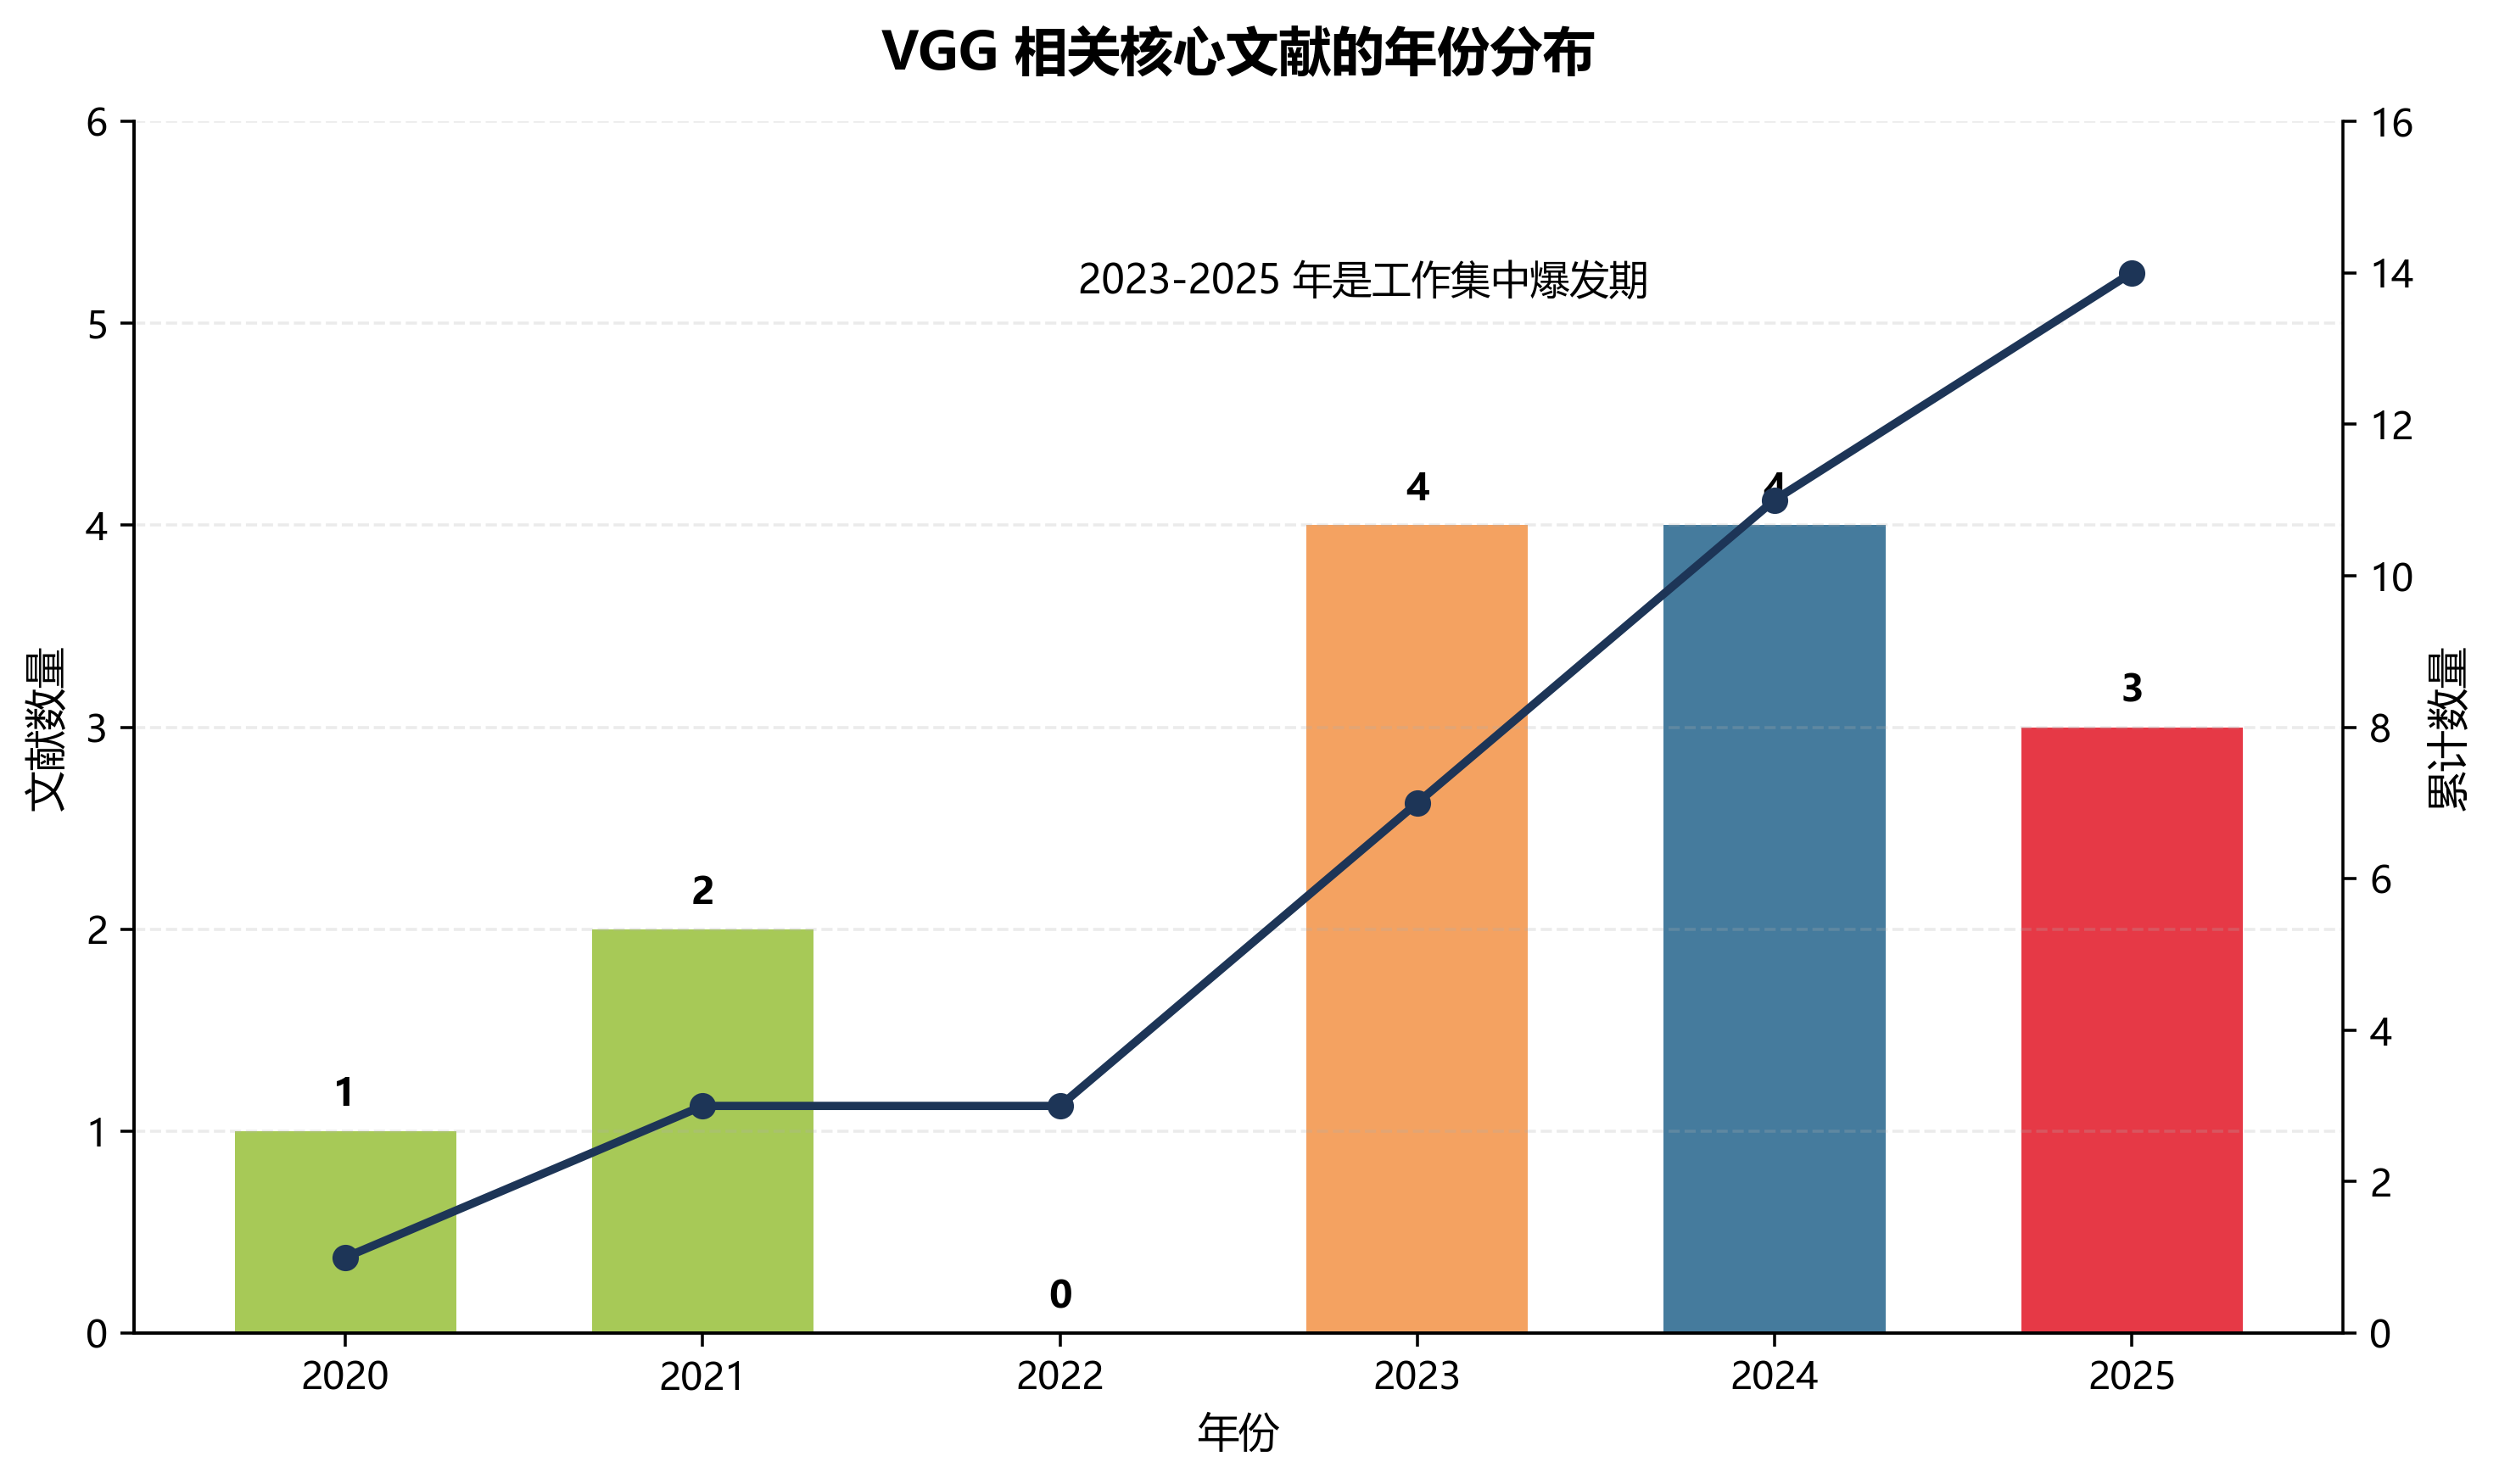
\includegraphics[width=10.8cm]{figures/vgg_year_distribution.png}
  \BiCaption{VGG 相关核心文献的年份分布}{Year-wise Distribution of Core VGG-related References}
  \label{fig:vgg-year-distribution}
\end{figure}

从文献时间分布上看，如图~\ref{fig:vgg-year-distribution} 所示，VGG 团队与本文主题直接相关的核心工作主要集中在 2023--2025 年。这一现象说明该研究方向并非长期稳定的传统子领域，而是在近几年随着 Transformer、点轨迹学习和统一几何预测方法的发展而快速升温。换言之，本文所综述的并不是一个已经完全定型的成熟方向，而是一条仍在快速延展、且研究范式仍在变化中的新兴主线。

如果进一步观察图中堆叠柱的内部构成，还可以发现数量增长并不是平均发生的，而是伴随着研究重心的阶段性迁移。2020--2021 年的代表工作主要集中在几何先验、任务设定与数据基础层面，说明该阶段的重点是回答“什么问题值得学、用什么数据来学、哪些几何结构不能丢”；2023--2024 年的新增工作则明显集中在对应关系和点轨迹建模上，说明团队开始优先修补传统管线中最脆弱的观测环节；直到 2024--2025 年，系统重构与统一输出相关工作才真正集中出现。这意味着 VGG 主线的推进并不是围绕单一模型持续做局部改良，而是沿着“观测—求解—表示”的问题链条不断上移。

\begin{figure}[H]
  \centering
  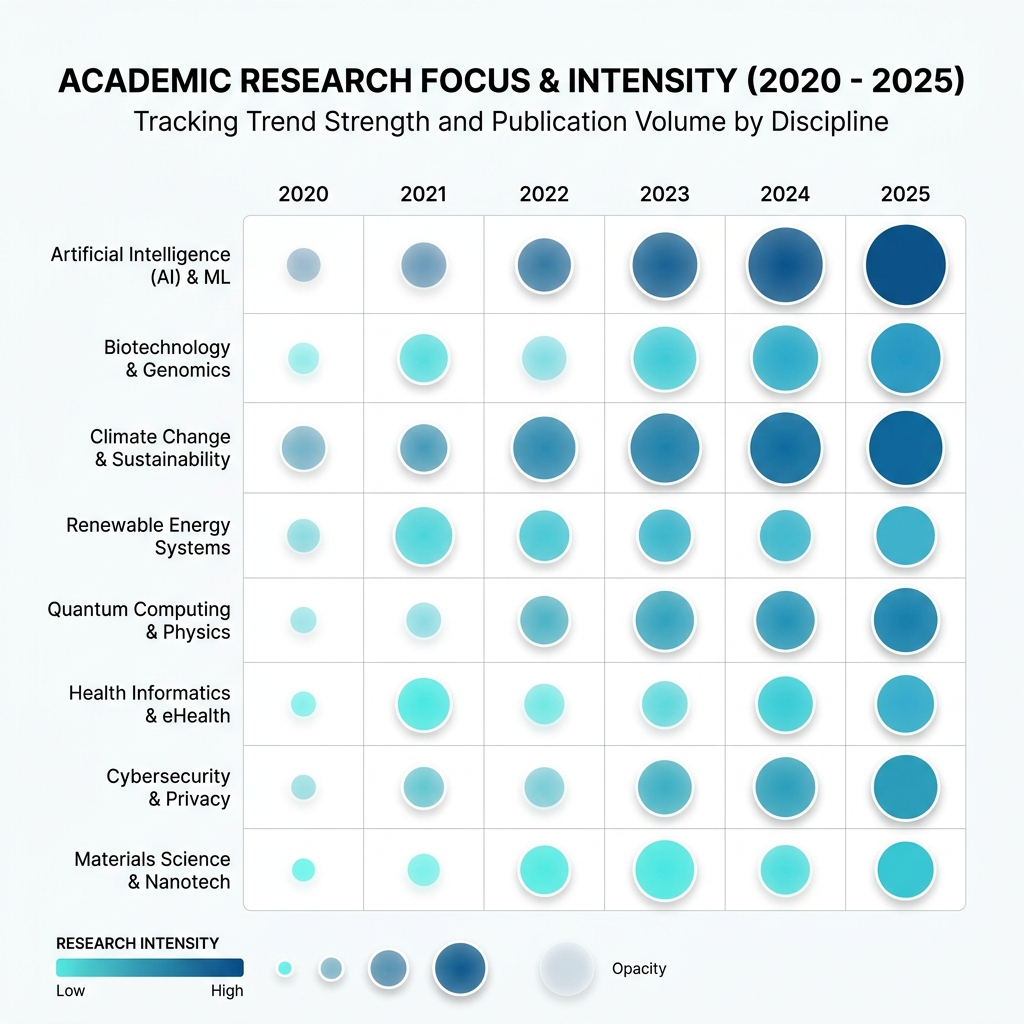
\includegraphics[width=11.2cm]{figures/vgg_focus_heatmap.png}
  \BiCaption{VGG 相关文献的研究重心分布热图}{Heatmap of Research Focus in Core VGG-related References}
  \label{fig:vgg-focus-heatmap}
\end{figure}

图~\ref{fig:vgg-focus-heatmap} 进一步把这种迁移关系表达得更清楚。若只看年份，读者可能会把这一主线理解为“近两年论文变多了”；但若结合研究重心类别，就会发现真正重要的变化在于论文所处理的问题层级发生了变化：早期更重视归纳偏置和数据基座，中期重视轨迹化观测与系统求解，后期则开始把统一几何表示和动态扩展纳入同一框架。按照课程报告对“研究思路如何逐步推进”的要求，这一点尤其关键，因为它解释了为什么本文不能简单按年份罗列文献，而必须按方法作用于管线的层次来组织。

\clearpage
\section{从经典几何到学习化建模的过渡}

\subsection{传统多视图几何重建范式}

传统多视图几何重建通常建立在 Structure-from-Motion（SfM）与 Multi-View Stereo（MVS）框架之上，其核心流程包括局部特征提取、跨图像匹配、几何验证、相机位姿恢复、三角化以及后续的全局优化\cite{triggs2000bundle,schoenberger2016colmap}。这一范式的优势在于几何解释清晰、优化目标明确，但同时也高度依赖局部描述子的稳定性与初始化质量。只要前端匹配失败，后续相机估计与重建质量往往会快速恶化。

经典管线的另一个特点是模块化程度高。前端负责提取与关联二维观测，后端则负责全局一致性优化。这种分治结构在工程实现上较为成熟，但也使得整个系统难以直接从最终重建误差中反向修正前端表征\cite{wang2024vggsfm}。随着深度学习方法在视觉任务中的广泛成功，研究者开始思考：能否让神经网络承担传统管线中最脆弱或最耗时的部分，同时保留多视图几何的结构性约束。

\subsection{学习方法为何进入多视图几何重建}

学习方法之所以逐步进入多视图几何重建，根本原因在于传统方法在复杂真实场景中的鲁棒性和泛化能力存在明显天花板。面对大视角变化、弱纹理、动态区域与复杂光照时，纯几何启发式往往难以稳定建立高质量对应\cite{wang2021deep2view}。而深度网络则能够从大规模数据中学习跨视角不变特征，并利用上下文提高匹配与估计质量。

不过，多视图几何重建的学习化并不意味着完全放弃几何结构。相反，该方向真正有效的工作通常强调“以几何为骨架、以学习为增强”的思路：学习模块负责估计更可靠的特征、轨迹或初始化，而多视图几何仍然提供问题定义、约束形式与评价标准\cite{bhalgat2023lighttouch,wang2024vggsfm}。从这一角度看，学习方法在该领域的发展更接近“重新组织几何管线”，而非“黑盒替代几何”。

\subsection{VGG 团队早期代表工作}

VGG 团队的早期工作体现出鲜明的过渡特征。首先，\textit{Unsupervised Learning of Probably Symmetric Deformable 3D Objects from Images in the Wild} 关注的是在弱监督条件下利用对称性等物理先验恢复三维结构，体现了“先验驱动学习”的思路\cite{wu2020unsup3d}。该工作虽然更接近单图重建，但它说明了几何与形状先验在学习式三维理解中的基础作用。

其次，\textit{Deep Two-View Structure-from-Motion Revisited} 则更加直接地讨论双视图结构恢复中哪些环节适合学习、哪些环节应保留经典几何求解\cite{wang2021deep2view}。该工作并未简单回归相机位姿或深度，而是将光流估计、相对位姿恢复和尺度不变深度估计有机组合，强调经典几何问题的可解性边界。这类工作为后续更系统的可微 SfM 研究奠定了方法论基础。

再次，\textit{Common Objects in 3D}（CO3D）数据集工作则从数据层面补齐了真实世界多视图学习的关键基础设施\cite{reizenstein2021co3d}。由于许多学习方法长期依赖合成数据或小规模真实数据，跨域泛化能力受限，CO3D 提供的大规模真实多视图对象数据集为后续研究提供了更接近真实场景的训练与评测基准。

\subsection{本综述的分析视角}

基于上述背景，本文后续不按论文年份简单罗列，而是按照学习方法逐步介入传统多视图几何管线的方式来组织。具体而言，本文将从“几何对应学习”“可微结构恢复”“统一前馈预测”三个层面梳理 VGG 团队的代表工作，并在必要处引入 DUSt3R 等相关方法作为横向对照\cite{wang2024dust3r}。

\clearpage
\section{几何对应学习与表征增强}

\subsection{几何先验如何进入 Transformer}

在多视图几何重建中，对应关系始终是最基础的输入信号。VGG 团队在这一问题上的一个关键思路，是将几何规律提前编码到表征学习过程中，而不是仅在后端优化阶段使用几何约束。\textit{A Light Touch Approach to Teaching Transformers Multi-View Geometry} 正是这一思路的代表\cite{bhalgat2023lighttouch}。该工作并不直接求解完整三维结构，而是研究如何通过极线几何去约束 Transformer 的跨视角注意力分布，使其更容易学习合理的跨图像关系。

这一思路的重要意义在于，它把几何从“解码时的硬约束”转化为“训练时的归纳偏置”。相比直接依赖大规模数据让模型自行发现几何结构，这种做法更符合多视图几何问题本身的物理规律，也为后续将 Transformer 用于更复杂的几何任务提供了方法启发\cite{wang2025vggt}。

\subsection{从成对匹配到点轨迹建模}

传统 SfM 更擅长处理成对匹配，再通过链接策略拼接成多视图轨迹。但在弱纹理、遮挡、长时序或视角变化较大时，这种做法容易引入链式误差。VGG 团队随后将研究重点推进到点轨迹学习，试图直接从视频或多帧图像中学习更稳定的时空对应表达。

\textit{DynamicStereo: Consistent Dynamic Depth From Stereo Videos} 关注动态场景中的深度一致性问题，说明了仅靠逐帧估计往往难以获得时间稳定的几何结果，因此需要显式建模时间维度上的几何关系\cite{karaev2023dynamicstereo}。这一工作虽然面向动态深度估计，但其核心价值在于强调“对应关系并非静态成对关系，而是时空一致性问题”。

在这一基础上，\textit{CoTracker: It is Better to Track Together} 进一步提出联合点追踪思想\cite{karaev2024cotracker}。与将每个点独立处理的追踪器不同，CoTracker 通过共享上下文、联合建模大量点轨迹，使模型能够更好地处理遮挡、出画与长时段追踪。对于多视图几何重建而言，这种轨迹形式具有重要意义，因为它提供了比传统稀疏匹配更稳定、更密集、更适合后续几何求解的观测基础。

\subsection{CoTracker3 与真实视频监督}

\textit{CoTracker3: Simpler and Better Point Tracking by Pseudo-Labelling Real Videos} 延续了轨迹建模思路，但重点转向如何更有效地利用真实视频数据\cite{karaev2025cotracker3}。该工作通过伪标签机制减少人工标注依赖，强化了模型在真实场景中的可迁移性与训练效率。对本文主题而言，其价值不只体现在追踪性能提升上，更在于说明高质量对应学习正在从“算法模块”变成“多视图几何系统的通用基础设施”。

\subsection{本阶段工作的主线作用}

从 Light Touch 到 CoTracker 系列，VGG 团队并未急于直接构建统一的三维重建模型，而是优先解决几何系统中最基础、最脆弱的输入问题：如何获得稳定可信的跨视角关系。这一阶段的研究成果为后续 VGGSfM 的全局相机恢复和可微优化提供了更强的底层观测，也解释了为何 VGG 团队的方法主线具有明显的递进性，而非彼此割裂的独立尝试。

\clearpage
\section{可微几何优化与端到端 SfM}

\subsection{从模块增强到系统级重构}

如果说对应学习解决的是前端观测质量问题，那么可微 SfM 则进一步触及传统多视图几何的核心系统结构。过去许多深度学习方法只替换匹配、深度或位姿初始化等局部模块，而后端仍沿用不可微的经典优化器。这使得系统难以真正实现端到端学习，也限制了最终误差对前端表征的反馈能力\cite{wang2021deep2view}。

\textit{VGGSfM: Visual Geometry Grounded Deep Structure From Motion} 在这方面迈出关键一步\cite{wang2024vggsfm}。该工作将深度点轨迹、相机恢复、三角化和 Bundle Adjustment 组织到同一可微框架中，使传统 SfM 系统中的多个关键环节能够在统一目标下训练。与仅对某个部件做学习增强的方案相比，VGGSfM 更接近对整个结构恢复问题的“系统级重构”。

\subsection{VGGSfM 的核心思想}

VGGSfM 的一个重要特点是同时强调“几何 grounded”与“深度学习驱动”。其输入不再是传统关键点匹配链，而是由点轨迹提供的更稳定观测；其相机恢复不是增量式逐步注册，而是尝试同步估计全部相机；其三维点优化则通过可微的 BA 层来完成\cite{wang2024vggsfm}。这意味着模型不仅在前端表征上使用学习方法，也在后端优化层面尽量保留传统几何问题的可解释形式。

从研究主线角度看，VGGSfM 是 VGG 团队从“增强几何管线”走向“重构几何管线”的转折点。一方面，它延续了前一阶段对轨迹、匹配和几何约束的重视；另一方面，它通过可微化方式将原本分离的多个模块组织到统一训练框架中，为进一步走向前馈式统一几何预测创造了条件。

\subsection{与传统 SfM 及同类方法的关系}

相较于 COLMAP 等传统系统，VGGSfM 的优势主要在于能够借助学习表征改善鲁棒性，并通过统一训练强化全局一致性\cite{schoenberger2016colmap,wang2024vggsfm}。相较于只在前端使用深度特征、后端仍完全依赖传统不可微求解器的混合方案，VGGSfM 则体现出更强的系统整合能力。

不过，VGGSfM 仍然保留了优化层，说明这一阶段的重点仍是“让几何优化可学习”，而非完全放弃优化。这一点在研究路径上十分关键：它既保留了传统几何的确定性和解释性，也暴露出后续研究进一步追求效率与统一性的方向，即能否在不依赖复杂测试时优化的前提下，直接输出关键三维属性。

\clearpage
\section{前馈式统一几何预测与方法趋势}

\subsection{从可微优化到统一前馈推断}

在可微 SfM 之后，VGG 团队研究主线继续向“统一化”与“前馈化”推进。\textit{VGGT: Visual Geometry Grounded Transformer} 提出以单个前馈网络直接预测相机参数、深度图、点图和三维点轨迹等关键几何属性，试图将传统多阶段系统进一步压缩为统一模型\cite{wang2025vggt}。这表明研究问题的表述已经从“如何提升某一几何模块”转向“如何以统一表示组织多个几何任务”。

VGGT 的意义不只在于预测速度更快，更在于它反映出多视图几何重建研究的一个重要趋势：学习模型开始承担传统后端优化原本负责的更大一部分工作。相比于需要测试时迭代求解的系统，前馈式方法在部署、复用和跨任务迁移上具有更高潜力\cite{wang2025vggt}。这也是 VGGT 被视为 VGG 团队研究主线阶段性代表作的重要原因。

\subsection{与相关方法的横向比较}

为了更好理解 VGGT 的定位，可以将其与 DUSt3R 等近期方法进行对照。DUSt3R 也强调从图像中直接恢复三维几何，并在一定程度上简化传统结构恢复流程\cite{wang2024dust3r}。但与 VGG 团队这一主线相比，VGGT 更强调统一的几何属性输出，以及与前述几何先验、轨迹学习和可微 SfM 研究的连续性。

此外，\textit{Splatter Image: Ultra-Fast Single-View 3D Reconstruction} 虽然聚焦单图重建，但它同样体现出 VGG 团队对“前馈式三维表示”的持续探索\cite{szymanowicz2024splatter}。这说明 VGG 团队并非只在传统多视图任务上推进学习化，也在尝试寻找更统一、更高效的三维表示方式。

\subsection{向动态几何与统一表示扩展}

这一趋势还继续延伸到动态几何场景。\textit{Dynamic Point Maps: A Versatile Representation for Dynamic 3D Reconstruction} 说明，当场景随时间变化时，统一点图表示仍可作为多任务几何建模的重要中间层\cite{sucar2025dpm}。尽管这类工作已部分超出本文“多视图几何重建”的核心范围，但它们揭示了一个清晰方向：未来的学习方法可能不再局限于重建某个静态结果，而是形成可支持深度、相机、点云、轨迹乃至动态场景理解的统一几何表征。

\subsection{本阶段的综合评价}

从 VGG 团队近五年的方法演进来看，前馈式统一几何预测并不是凭空出现的，而是建立在前述几何先验注入、点轨迹学习与可微 SfM 逐步成熟的基础之上。也正因为如此，VGGT 等方法更适合被理解为一条研究主线的阶段性总结，而不是孤立的单篇突破。对本文主题而言，本阶段最值得强调的不是单个模型的性能，而是“多视图几何重建正在从优化驱动转向表示驱动与模型驱动”的方法论变化。

\clearpage
\section{总结与展望}

本文围绕“多视图几何重建中的学习方法”这一主题，以 VGG 团队为例梳理了近五年的代表性研究主线。综合全文可以看到，VGG 团队的重要性并不只在于若干单篇论文分别提升了某项局部性能，而在于其成果之间形成了一条较完整、可解释的研究链：先以几何先验、数据基础与任务边界回答“学习方法能否真正进入几何问题”，再以点轨迹和对应学习回答“系统应当依赖什么样的观测”，随后以可微 SfM 回答“几何求解如何被重组为可学习系统”，最后以 VGGT 等工作进一步追问“统一表示能否吸收更多后端逻辑”\cite{wu2020unsup3d,wang2021deep2view,reizenstein2021co3d,bhalgat2023lighttouch,karaev2024cotracker,wang2024vggsfm,wang2025vggt}。因此，VGG 团队的研究不是若干论文的并列堆叠，而是一条由问题设定、观测组织、系统求解到表示统一逐步展开的清晰主线。

从研究特色上看，VGG 团队至少表现出四方面鲜明特点。第一，它始终以多视图几何中的可解结构为中心，而不是把三维重建理解为一般性的黑盒回归任务。第二，它强调系统级推进，不满足于只优化某个局部模块，而是不断重新组织观测、求解与表示之间的关系。第三，它重视真实数据、伪标签与基准构建，使研究主线不仅有方法创新，也有训练和评测基础设施的持续支撑\cite{reizenstein2021co3d,karaev2025cotracker3}。第四，它对统一几何表示保持持续关注，使模型输出不只服务于单次重建，而是逐步具备跨任务复用的潜力\cite{wang2025vggt,sucar2025dpm}。这些特点共同决定了 VGG 团队在该领域中的位置：它既不是完全站在传统 SfM 一侧，也不是简单站在“去几何化”的纯前馈路线一侧，而是处在“保留几何结构、同时推动学习化系统重构”的关键交汇点。

从对领域发展的推动作用看，VGG 团队的贡献主要体现在三个层面。其一，在观测层面，它推动研究者重新理解高质量对应的含义，使对应关系从脆弱的成对匹配逐步转向更稳定、更密集、可跨时空延续的轨迹表示\cite{bhalgat2023lighttouch,karaev2023dynamicstereo,karaev2024cotracker}。其二，在系统层面，它通过 VGGSfM 证明传统结构恢复并非只能依赖分散的不可微模块，而可以被重写为端到端可训练、可整体优化的几何系统\cite{wang2024vggsfm}。其三，在表示层面，它通过 VGGT 与 Dynamic Point Maps 等工作推动多视图几何从“优化驱动的流水线”进一步走向“表示驱动的统一建模框架”\cite{wang2025vggt,sucar2025dpm}。换言之，VGG 团队推动的不只是某个 benchmark 指标的上升，更是整个方向从模块增强走向系统重构、再走向统一表示的范式迁移。也正是在这个意义上，VGG 团队可以被视为当前多视图几何学习化进程中的代表性团队之一。

如果给出本文对其研究体系的整体评价，我更倾向于把 VGG 团队理解为当前多视图几何学习化进程中的“代表性中轴”。其优势在于推进路径稳健、问题意识清楚、前后工作衔接自然，因而特别适合用来观察这一方向如何从模块增强逐渐走向系统重构与统一表示。更重要的是，这一研究体系并没有脱离几何问题本身，而是在每一步都围绕“几何结构如何被保留、吸收和重用”这一核心矛盾展开。与此同时，这条主线也保留了值得继续警惕的张力：统一前馈模型虽然提高了效率与接口一致性，但也显著增强了对训练数据规模、监督质量和模型容量的依赖；而几何可解释性虽然仍被保留为重要目标，却尚未在动态、长尾和复杂开放场景中彻底转化为稳定优势\cite{wang2024vggsfm,wang2025vggt}。因此，对 VGG 主线最准确的评价不是“已经给出最终答案”，而是“较清楚地指明了下一阶段问题会出现在哪里”。

结合全文分析，本文最终想强调的综合结论是：多视图几何重建中的学习方法并没有削弱几何本身的重要性，反而促使几何约束以更灵活、更深层的形式进入特征学习、监督构造、系统设计与统一表示之中。VGG 团队之所以值得被单独综述，也正是因为它较完整地展示了这一变化过程。面向后续发展，可以预见该方向仍会围绕三个问题继续推进：其一，如何在减少显式优化的同时保持高精度和强可解释性；其二，如何利用更大规模真实数据与弱监督信号提升统一模型的泛化能力；其三，如何把当前以静态场景为主的统一几何表示进一步扩展到动态场景、开放世界感知与三维内容生成等更复杂任务中。总体而言，VGG 团队的研究体系尚未封闭，但其已经为这一方向的下一阶段演进给出了较清晰的路径指示。


\clearpage
\printbibliography[heading=custombib,title={参考文献}]

\end{document}
